\documentclass[11pt]{article}

\usepackage[margin=1in]{geometry}
\usepackage[T1]{fontenc}
\usepackage[utf8]{inputenc}
\usepackage{newtxtext,newtxmath}
\usepackage{microtype}
\usepackage{setspace}
\usepackage{amsmath,mathtools}
\usepackage{booktabs,tabularx,longtable,array}
\usepackage{graphicx}
\usepackage{xcolor}
\usepackage{caption}
\usepackage{enumitem}
\usepackage{listings}
\usepackage{needspace}
\usepackage{natbib}
\usepackage{hyperref}
\usepackage[nameinlink,noabbrev]{cleveref}
\usepackage{fancyhdr}

\definecolor{ferankblue}{HTML}{2F6B9A}
\definecolor{ferankorange}{HTML}{D77A2B}
\definecolor{ferankink}{HTML}{243447}
\definecolor{feranklight}{HTML}{EFF4F7}
\hypersetup{
  colorlinks=true,
  linkcolor=ferankblue,
  citecolor=ferankblue,
  urlcolor=ferankblue,
  pdftitle={Firm Rankings from Worker Flows: A Technical Guide to ferank},
  pdfauthor={Johannes F. Schmieder}
}

\newcolumntype{L}[1]{>{\raggedright\arraybackslash}p{#1}}
\newcolumntype{R}[1]{>{\raggedleft\arraybackslash}p{#1}}
\newcolumntype{Y}{>{\raggedright\arraybackslash}X}
\setlength{\tabcolsep}{5pt}
\setlength{\parindent}{0pt}
\setlength{\parskip}{0.55em}
\setstretch{1.05}
\setlist{nosep,leftmargin=1.5em}
\captionsetup{font=small,labelfont=bf}
\graphicspath{{generated/}}

\lstdefinelanguage{Stata}{
  morekeywords={use,clear,import,delimited,rename,keep,isid,ferank,worker,time,method,maxgap,component,normalize,tolerance,maxiter,threads,frame,replace,estat,convergence,components,list,sort,merge,generate,export},
  sensitive=false,
  morecomment=[l]{*},
  morecomment=[l]{//},
  morestring=[b]"
}
\lstset{
  language=Stata,
  basicstyle=\ttfamily\small,
  keywordstyle=\color{ferankblue}\bfseries,
  commentstyle=\color{gray},
  showstringspaces=false,
  frame=single,
  rulecolor=\color{feranklight},
  backgroundcolor=\color{feranklight},
  breaklines=true,
  columns=fullflexible,
  xleftmargin=0.5em,
  framexleftmargin=0.5em
}

\pagestyle{fancy}
\fancyhf{}
\fancyhead[L]{\small Technical guide to \texttt{ferank}}
\fancyhead[R]{\small Worker-flow rankings}
\fancyfoot[C]{\thepage}
\renewcommand{\headrulewidth}{0.3pt}

\newcommand{\VenetoRows}{71,614}
\newcommand{\VenetoWorkers}{35,807}
\newcommand{\VenetoRawFirms}{5,301}
\newcommand{\VenetoMoves}{8,243}
\newcommand{\VenetoSameFirm}{27,564}
\newcommand{\VenetoEdges}{6,043}
\newcommand{\VenetoGraphFirms}{3,630}
\newcommand{\VenetoLargestSCC}{702}
\newcommand{\VenetoSelectedMoves}{2,602}
\newcommand{\VenetoSelectedEdges}{2,010}
\newcommand{\VenetoMeanChange}{0.0196}
\newcommand{\VenetoSDChange}{0.2116}
\newcommand{\AkmRows}{20,584}
\newcommand{\AkmMovers}{2,602}
\newcommand{\AkmPeriodEffect}{0.0166}
\newcommand{\AkmRSquared}{0.094}
\newcommand{\AkmIterations}{45}
\newcommand{\NetworkNodes}{24}
\newcommand{\NetworkEdges}{55}
\newcommand{\SorkinBtSpearman}{0.792}
\newcommand{\SorkinAkmSpearman}{0.004}
\newcommand{\BtAkmSpearman}{-0.045}


\title{\vspace{-2em}\textbf{Firm Rankings from Worker Flows}\\[0.35em]
  \Large A Technical Guide to \texttt{ferank}}
\author{Johannes F. Schmieder}
\date{Version 0.1 companion report\\28 August 2026}

\begin{document}
\maketitle

\begin{abstract}
\noindent
\texttt{ferank} constructs firm rankings from the direction and frequency of
worker moves. This report is written for labor economists who know the
Abowd--Kramarz--Margolis (AKM) framework but do not use graph-theoretic
terminology. It develops the relevant graph concepts from first principles,
shows why direction and strong connectivity matter, derives the Sorkin and
Bradley--Terry estimators implemented by the command, and explains the input,
output, normalization, diagnostics, and failure behavior. A reproducible
application uses the public Veneto-based teaching extract distributed with
\texttt{LeaveOutKSS}. The example has \VenetoWorkers{} workers and
\VenetoRows{} worker-year rows. Its largest strongly connected firm component
contains \VenetoLargestSCC{} firms. The example is deliberately descriptive:
the command supplies point rankings from worker flows, not wage effects,
standard errors, amenities, rents, or causal employer values.
\end{abstract}

\vspace{0.4em}
\colorbox{feranklight}{\begin{minipage}{0.95\linewidth}\small
\textbf{The central translation for an AKM reader.}
AKM asks which firm effects can be compared through workers who connect firms.
\texttt{ferank} instead asks which firms are favored by the \emph{direction}
of those connections. A worker who moves from firm $j$ to firm $i$ creates an
arrow $j\rightarrow i$. The two estimators turn the resulting system of arrows
into a scalar score for each firm. The estimand is therefore about revealed
worker flows, even when the data also contain earnings.
\end{minipage}}

\tableofcontents
\newpage

\section{What the command estimates}
\label{sec:estimand}

Let $w$ index workers, $t$ time, and $J_{wt}$ the employer observed for worker
$w$ at $t$. Whenever two consecutive valid observations show
$J_{w,t^-}=j$ and $J_{wt}=i\neq j$, the data contain a directed move from the
\emph{origin} $j$ to the \emph{destination} $i$. Aggregating such events gives
the flow matrix
\begin{equation}
  M_{ij}=\text{number (or weight) of observed moves from firm $j$ to firm $i$}.
  \label{eq:flowmatrix}
\end{equation}
The destination index is the row and the origin index is the column. This
orientation is worth fixing at the outset: it determines every formula and it
makes the destination the ``winner'' in the Bradley--Terry estimator.

Both methods implemented by \texttt{ferank} consume exactly the same canonical
positive-flow edges $(j,i,M_{ij})$:
\begin{itemize}
  \item \textbf{Sorkin} follows flows through the entire network and reports
  the stationary revealed value associated with each firm
  \citep{sorkin2018ranking}.
  \item \textbf{Bradley--Terry} treats every $j\rightarrow i$ move as a paired
  comparison that destination $i$ wins against origin $j$
  \citep{bradley1952rank}.
\end{itemize}
Higher scores receive better ranks: rank 1 is best. The two methods need not agree because
Sorkin uses global propagation through all paths, whereas Bradley--Terry asks
how destinations perform conditional on the firm pairs that workers compare.

\subsection{What it does not estimate}

An AKM wage equation is commonly written
\begin{equation}
  y_{wt}=\alpha_w+\psi_{J_{wt}}+x_{wt}'\beta+\varepsilon_{wt},
  \label{eq:akm}
\end{equation}
where $\psi_j$ is a firm effect on the outcome after controlling for worker
heterogeneity and observables \citep{abowd1999highwage}. In contrast,
\texttt{ferank} never uses $y_{wt}$. It does not estimate $\psi_j$, nor does it
automatically interpret worker mobility as exogenous. It also does not return
standard errors, confidence intervals, offer shares, amenities, rents, or
structural utility. A flow ranking can be related to an AKM firm effect in a
separate analysis, but equality between the two objects is neither imposed nor
expected.

\section{Graph theory in labor-economics language}
\label{sec:graph}

A \emph{graph} is simply a bookkeeping device for objects and relationships.
Here the objects are firms and the relationships are worker moves. The formal
vocabulary is useful because it states precisely which comparisons the data
support.

\begin{figure}[htbp]
  \centering
  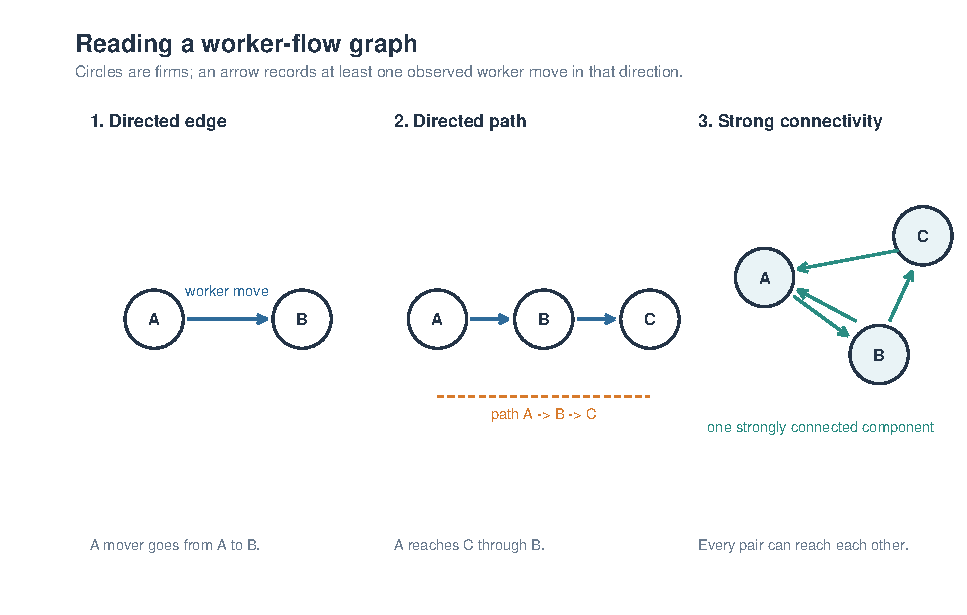
\includegraphics[width=\linewidth]{graph_concepts.pdf}
  \caption{The three pieces of graph language used most often in this report.
  Direction is substantive: the existence of $A\rightarrow B$ does not imply
  $B\rightarrow A$.}
  \label{fig:concepts}
\end{figure}

\subsection{Vertices, directed edges, weights, and degrees}

The following terms translate directly into linked employer--employee data.
\begin{table}[htbp]
\centering
\caption{Graph terminology translated into the worker-flow setting}
\label{tab:glossary}
\small
\begin{tabularx}{\linewidth}{@{}L{0.19\linewidth}L{0.28\linewidth}Y@{}}
\toprule
Term & Formal meaning & Meaning in \texttt{ferank} \\
\midrule
Vertex (node) & An object in the graph & A firm identifier that appears in at least one positive cross-firm move \\
Directed edge & An ordered pair $j\rightarrow i$ & At least one worker moves from origin $j$ to destination $i$ \\
Edge weight & A nonnegative number attached to an edge & The number or supplied weight of moves $M_{ij}$ after duplicate rows are aggregated \\
Inflow / outflow & Total weight entering / leaving a vertex & $\sum_j M_{ij}$ / $\sum_i M_{ij}$ for a firm \\
In-degree / out-degree & Number of distinct incoming / outgoing neighbors & How many distinct firms send workers to / receive workers from the firm \\
Directed path & A sequence of arrows whose heads and tails line up & A chain such as $A\rightarrow B\rightarrow C$; no worker need traverse the entire chain \\
Reachability & Existence of at least one directed path & Firm $C$ is reachable from $A$ if some chain of observed move directions leads from $A$ to $C$ \\
Strongly connected & Each vertex can reach every other vertex in both directions & Every partition of the firms is crossed by worker flows in the directions needed for a finite common ranking \\
Strongly connected component (SCC) & A maximal strongly connected subset & A largest group that satisfies the preceding condition; groups are maximal, so none can be enlarged \\
Laplacian & A matrix of local differences along graph edges & The curvature matrix in a Bradley--Terry Newton step, with one uninformative constant direction \\
\bottomrule
\end{tabularx}
\end{table}

A direction-free AKM connected set and a directed SCC are not the same object.
For AKM identification, one usually asks whether the underlying worker--firm
links connect firm effects up to a normalization \citep{abowd2002computing}.
If one erases all arrows in a flow graph, the remaining undirected graph may be
connected even when the directed graph is not strongly connected. For example,
$A\rightarrow B\rightarrow C$ connects all three firms after directions are
erased, but there is no directed route back from $C$ to $A$.

\subsection{Paths are chains of evidence, not worker histories}

A directed path $A\rightarrow B\rightarrow C$ means only that the data contain
an $A$-to-$B$ move and a $B$-to-$C$ move. They may be made by different
workers and at different dates. Paths allow local directional comparisons to
propagate globally. In Sorkin, probability mass travels along them. In
Bradley--Terry, overlapping pair comparisons connect score differences.

\subsection{Why strong connectivity is the estimation boundary}
\label{subsec:scc}

A set is strongly connected if, for every firms $i$ and $j$, there is a
directed path from $i$ to $j$ \emph{and} a directed path from $j$ to $i$.
The SCCs partition the positive-flow graph and can be found in time
proportional to vertices plus edges using depth-first-search algorithms such as
\citet{tarjan1972depth}.

Strong connectivity matters for both estimators:
\begin{enumerate}
  \item For Sorkin it makes the flow transition matrix irreducible, delivering
  a unique positive stationary distribution after normalization
  \citep{levin2017markov}.
  \item For Bradley--Terry it is the comparison-graph condition that rules out
  a direction of complete separation and permits a finite maximum-likelihood
  estimate \citep{ford1957solution}.
\end{enumerate}
The command therefore never invents comparability. It does not join SCCs with
teleportation, a ridge penalty, pseudo-moves, or hidden smoothing. Under
\texttt{component(all)}, separate SCCs get separate normalizations, so their
score levels and ranks are not comparable across components.

\section{From panel records to one canonical mobility graph}
\label{sec:construction}

\texttt{ferank} accepts either a worker--firm panel or a prepared edge list.
The two routes meet at one canonical edge representation.

\subsection{Panel mode}

Panel mode first restricts the sample using any \texttt{if} or \texttt{in},
then requires exactly one firm per worker--time pair. It orders observations
internally. Two consecutive valid records generate a unit move only if:
\begin{enumerate}
  \item the worker identifier agrees;
  \item the time difference is positive and no larger than
  \texttt{maxgap(\#)}; and
  \item origin and destination firms are both observed and differ.
\end{enumerate}
A same-firm pair is counted as a continuation, not a self-edge. A missing firm
breaks the worker's transition chain. Duplicate worker--time records are an
error because the command will not choose a dominant job or split a worker
across concurrent jobs. Researchers must resolve multiple jobs, nonemployment,
recalls, spell rules, and fractional moves before estimation if those choices
matter for the application.

\subsection{Prepared-edge mode}

Prepared-edge mode takes origin and destination variables and an optional
\texttt{flow()} weight. The default weight is one. The command rejects negative
or nonfinite weights, excludes zero weights and self-moves, sorts directed
pairs deterministically, aggregates duplicates using compensated summation,
and then applies \texttt{minflow()}. Applying the threshold after aggregation
ensures that splitting one edge across input rows cannot alter inclusion.

\subsection{Canonicalization and component selection}

After either input route, the canonical graph has one positive row per
directed firm pair. SCCs are computed before estimation.
\texttt{component(largest)} chooses the SCC with the most firms; ties are
broken by retained flow and then by the smallest firm identifier.
\texttt{component(\#)} chooses a reported component number, and
\texttt{component(all)} estimates all qualifying SCCs separately.

\section{The Sorkin revealed-preference fixed point}
\label{sec:sorkin}

The Sorkin estimator turns employer-to-employer moves into a revealed-preference
ranking \citep{sorkin2018ranking}. Define firm $j$'s total outflow
\begin{equation}
  s_j=\sum_i M_{ij}, \qquad S=\operatorname{diag}(s_1,\ldots,s_J),
\end{equation}
and the column-stochastic transition matrix
\begin{equation}
  P=MS^{-1}, \qquad P_{ij}=\frac{M_{ij}}{s_j}.
  \label{eq:transition}
\end{equation}
$P_{ij}$ is the observed share of moves leaving $j$ that go to $i$. A
stationary mass vector $\pi$ solves
\begin{equation}
  P\pi=\pi, \qquad \mathbf{1}'\pi=1.
  \label{eq:stationary}
\end{equation}
The equation asks for a distribution of mass over firms that is unchanged
after mass follows observed move shares once. This is the same mathematical
object called a stationary distribution in Markov-chain language, but no
behavioral claim that an individual worker literally follows a Markov process
is required to compute the descriptive fixed point.

Stationary mass alone is mechanically larger at firms with more departures.
The revealed value divides this exposure back out:
\begin{equation}
  q=S^{-1}\pi, \qquad q_j=\frac{\pi_j}{s_j}.
  \label{eq:q}
\end{equation}
\texttt{ferank} reports $\log q_j$ after an additive normalization. A firm can
therefore rank highly because the complete system sends disproportionate
stationary mass to it relative to the amount of flow leaving it. This is a
global statement: paths through third firms matter.

\subsection{Why the iteration is made lazy}

If moves form an exact cycle, ordinary power iteration on $P$ can oscillate
even though the stationary distribution is well-defined. Production uses
\begin{equation}
  \widetilde P=(1-\lambda)I+\lambda P,
  \qquad 0<\lambda\leq 1,
  \label{eq:lazy}
\end{equation}
with \texttt{lazy(0.5)} by default. The self-loop makes the numerical iteration
aperiodic while leaving every solution of \cref{eq:stationary} unchanged. This
is a numerical device, not teleportation and not an extra observed flow.

\subsection{What certifies convergence}

Small change between two iterations can be misleading for nearly reducible
graphs. \texttt{ferank} evaluates the accepted $\pi$ against the original,
non-lazy equation. It requires both
\begin{equation}
  \lVert P\pi-\pi\rVert_{\infty}\leq\texttt{tolerance()}
  \quad\text{and}\quad
  \lVert P\pi-\pi\rVert_{1}\leq\texttt{tolerance()},
\end{equation}
plus agreement with an alternative starting vector at a score gate based on
$\sqrt{\texttt{tolerance()}}$. The command stores the maximum and L1
residual norms in \texttt{e()}; firm-level signed residuals are not published
as output variables.

\section{The Bradley--Terry paired-comparison ranking}
\label{sec:bt}

Bradley--Terry assigns each firm a real-valued score $\theta_i$. Conditional on
a comparison between firms $i$ and $j$, the model writes
\begin{equation}
  \Pr(i\text{ wins against }j)
  =\sigma(\theta_i-\theta_j)
  =\frac{\exp(\theta_i-\theta_j)}{1+\exp(\theta_i-\theta_j)}.
  \label{eq:btprob}
\end{equation}
In the mobility application, a move $j\rightarrow i$ is a win for destination
$i$. Thus the weighted log likelihood is
\begin{equation}
  \ell(\theta)=\sum_{i\neq j}M_{ij}
  \log\sigma(\theta_i-\theta_j).
  \label{eq:btll}
\end{equation}
The formulation is a ranking model for directed moves. It does not claim that
the worker chose from exactly two simultaneous offers; ``paired comparison''
describes the statistical likelihood, not a complete search model.

For the unordered pair $\{i,j\}$, let $n_{ij}=M_{ij}+M_{ji}$. The score equation
for firm $i$ has the intuitive observed-minus-predicted form
\begin{equation}
  g_i(\theta)=\sum_{j\neq i}
  \left[M_{ij}-n_{ij}\sigma(\theta_i-\theta_j)\right]=0.
  \label{eq:btgradient}
\end{equation}
Increasing $\theta_i$ raises the predicted share of comparisons won by $i$.
The maximum balances actual destination wins against those predicted from all
of $i$'s pairwise score gaps.

\subsection{The Laplacian, explained without graph prerequisites}

The negative Hessian of \cref{eq:btll} is a weighted graph Laplacian. For each
compared pair, the weight is
\begin{equation}
  w_{ij}(\theta)=n_{ij}\,p_{ij}(1-p_{ij}),
  \qquad p_{ij}=\sigma(\theta_i-\theta_j).
\end{equation}
The Laplacian puts $\sum_j w_{ij}$ on diagonal element $i$ and $-w_{ij}$ on
off-diagonal element $(i,j)$. For any vector $x$,
\begin{equation}
  x'Lx=\sum_{i<j}w_{ij}(x_i-x_j)^2.
  \label{eq:laplacian}
\end{equation}
This identity is all an applied reader needs: curvature is information about
\emph{score differences along observed comparison links}. Adding the same
constant to every score changes no difference, so $L\mathbf{1}=0$. A
normalization removes this single uninformative direction.

\subsection{Newton/IRLS computation and certificates}

The production solver uses overflow-safe likelihood evaluation and
Newton/iteratively reweighted least squares. Each Newton step solves a
Laplacian linear system on the mean-zero subspace. Bounded systems use a dense
augmented KKT solve; larger systems use preconditioned conjugate gradients with
the repository's audited combinatorial-multigrid adapter. An ascent-preserving
line search rejects steps that reduce the likelihood.

Acceptance requires a small constrained gradient, a small Newton-system
residual, and stable likelihood. Strong connectivity is checked before
optimization, so separation is an error rather than a falsely converged
infinite score. \texttt{estat convergence} exposes these quantities and the
linear-solver route.

\section{Normalization, ranks, and interpretation}
\label{sec:normalization}

Both objectives identify relative scores. The following normalizations shift
every score in a component by the same constant and therefore leave fitted
comparisons and ranks unchanged:
\begin{itemize}
  \item \texttt{normalize(mean)} sets the unweighted component mean to zero;
  \item \texttt{normalize(weighted)} sets a user-weighted mean to zero and
  requires \texttt{normweight()} to be constant within firm; and
  \item \texttt{normalize(reference)} sets the firm supplied in
  \texttt{reference()} to zero.
\end{itemize}
Higher scores receive better ranks: rank 1 is best. Exact numerical ties receive the same
deterministic midrank and percentile; firm identifiers order output rows but
never break an econometric tie. Scores in different SCCs remain incomparable
even if each is mean-normalized.

The most defensible language is ``a higher Sorkin revealed-flow value'' or ``a
higher Bradley--Terry worker-flow ranking.'' Calling either score a wage premium,
firm productivity, amenity, rent, or causal value requires assumptions and
evidence outside this command.

\section{Command syntax and option-by-option behavior}
\label{sec:syntax}

\subsection{Two input modes}

\begin{lstlisting}
* Prepared directed edges
ferank origin destination [if] [in], method(sorkin|bradleyterry) ///
    generate(origin_rank destination_rank) [flow(weight) options]

* Worker-firm panel
ferank firm [if] [in], worker(worker_id) time(period) ///
    method(sorkin|bradleyterry) generate(firm_rank) [options]
\end{lstlisting}

{\small
\begin{longtable}{@{}L{0.30\linewidth}L{0.62\linewidth}@{}}
\caption{Options in version 0.1}\label{tab:options}\\
\toprule
Option & Meaning and practical implication \\
\midrule
\endfirsthead
\toprule
Option & Meaning and practical implication \\
\midrule
\endhead
\texttt{method()} & Required. Chooses \texttt{sorkin} or \texttt{bradleyterry}. Both use the same canonical graph. \\
\texttt{flow(varname)} & Prepared-edge mode only. Supplies nonnegative edge weight; the default is one per input row. \\
\texttt{worker()}, \texttt{time()} & Panel mode only and both required. Identify worker histories and order observations. \\
\texttt{maxgap(\#)} & Panel mode. Largest allowed time difference between consecutive records; default 1. A gap beyond the limit breaks the transition. Units are those of \texttt{time()}. \\
\texttt{component(largest|\#|all)} & Chooses the largest SCC (default), a reported SCC number, or all qualifying SCCs separately. \\
\texttt{normalize(mean|}\linebreak\texttt{weighted|reference)} & Additive score normalization; default mean. \\
\texttt{normweight(varname)} & Required for weighted normalization. Must be nonnegative and constant within firm. \\
\texttt{reference(\#)} & Required for reference normalization. Identifies the firm whose score is set to zero. \\
\texttt{minflow(\#)} & Drops canonical edges with aggregated flow below the threshold. Default 0. Changing it can change SCC membership. \\
\texttt{tolerance(\#)} & Numerical certificate tolerance; default $10^{-10}$. It governs original-equation residual checks, not merely iteration change. \\
\texttt{maxiter(\#)} & Maximum outer iterations; default 20,000. Reaching the limit without a certificate is an error. \\
\texttt{threads(\#)} & Requests deterministic native worker threads. Zero lets the plugin choose. \\
\texttt{lazy(\#)} & Sorkin only. Weight $\lambda\in(0,1]$ in \cref{eq:lazy}; default 0.5. It changes convergence behavior, not the target stationary vector. \\
\texttt{engine(plugin|reference)} & Uses the production sparse plugin or a bounded, separately implemented dense reference engine. \\
\texttt{generate(newvars)} & Ordinal midrank, with 1 best and average ranks for exact ties. \\
\texttt{score(newvars)} & Continuous normalized score; higher is better. Use for Pearson comparisons with AKM effects. \\
\texttt{percentile(newvars)} & Equal-firm percentile within each component; 100 is best. \\
\texttt{componentid(newvars)} & Deterministic estimated component ID, useful with \texttt{component(all)}. \\
\texttt{verbose} & Also displays the full method-specific convergence certificate. \\
\bottomrule
\end{longtable}
}

At least one of \texttt{generate()}, \texttt{score()}, or
\texttt{percentile()} is required. Each supplied output option takes one
new variable name in panel mode or two in prepared-flow mode, in
origin--destination order. Names must be distinct and new. The command adds
only those variables, preserving existing data, observation order and the
active frame; it creates no result frame. Older \texttt{frame()} and
\texttt{replace} calls must be migrated to named variable outputs.

The \texttt{if}/\texttt{in} restrictions select rows for both constructing
flows and filling outputs. Other rows stay missing, even when their firm is
ranked elsewhere. Selected panel rows receive their employer's estimate,
including terminal observations and workers who never move. Firms outside
selected components and missing employers receive missing values. In flow
mode the two endpoints are mapped independently; a self-move or zero-flow
row can receive values even though it contributes no comparison.

The main display separates full-graph counts from selected firms and mapped
rows, names every output variable, and reports convergence and native timing.
These native timings exclude Stata preparation and matching; use a timer
around the complete command for end-to-end performance. \texttt{e(N\_mapped)}
counts selected panel rows with a ranked firm, or flow rows with both firms
ranked. There is no observation-level \texttt{e(sample)} indicator.

Useful postestimation commands for a panel are:
\begin{lstlisting}
estat convergence   // numerical certificate for the method just run
estat components    // component rule, graph coverage and mapped rows
list firm firm_rank if firm_rank<=10
\end{lstlisting}

Firm values repeat across worker-year observations. Correlations on these
rows therefore weight firms by their matched person-years. For an equal-firm
comparison, keep one matched observation per firm. Score centering does not
change this distinction or the equal-firm percentile definition.

\subsection{Failure behavior is part of the scientific contract}

The command stops rather than guessing when it encounters duplicate
worker--time observations, mixed identifier storage types in edge mode,
negative or nonfinite flows, invalid normalization weights, an absent reference
firm, a requested component that does not qualify, a non-strong comparison
graph for the selected estimate, separation, or a failed numerical certificate.
All requested values are staged privately and published together only
after successful estimation and matching. A failed call leaves existing
data unchanged and creates no partial output variables.

\section{Worked Veneto example}
\label{sec:veneto}

\subsection{Data provenance and scope}

The replication uses the public example distributed with version 0.1.0 of the
R package \texttt{LeaveOutKSS} \citep{leaveoutkss2026}. The file is a small,
pseudonymous, Veneto-based teaching extract related to the leave-out variance
component application of \citet{kline2020leaveout}. It is \emph{not} the full
confidential Veneto Workers History analysis sample. The report therefore uses
only aggregate statistics and replaces pseudonymous firm identifiers with plot
aliases in the network figure.

The extract has ten numeric columns. The replication uses only the first four:
pseudonymous worker, pseudonymous firm, year, and the supplied outcome in its
original scale. \texttt{ferank} itself uses only the first three. The staging
script normalizes line endings and requires SHA-256
\begin{center}
\small\texttt{93e57a413a8cfccdcb043c5d793105a67b2dc9ebd27d5d3a4f1800abf89a2241}.
\end{center}

\subsection{The critical time-gap choice}

Every worker is observed in 1999 and 2001. The time variable therefore jumps
by two. The command's default \texttt{maxgap(1)} would correctly form zero
transitions. The empirical example must use \texttt{maxgap(2)}. This is not a
cosmetic option: \texttt{maxgap()} is expressed in the units of the supplied
time variable.

\Needspace{24\baselineskip}
\begin{lstlisting}
import delimited using "kss_example_1999_2001.csv", ///
    varnames(nonames) clear
rename v1 worker
rename v2 firm
rename v3 year
rename v4 outcome
keep worker firm year outcome
isid worker year

ferank firm, worker(worker) time(year) method(sorkin) ///
    maxgap(2) component(largest) normalize(mean) ///
    tolerance(1e-10) maxiter(20000) threads(8) ///
    generate(sorkin_rank) score(sorkin_score) percentile(sorkin_pct)

ferank firm, worker(worker) time(year) method(bradleyterry) ///
    maxgap(2) component(largest) normalize(mean) ///
    tolerance(1e-10) maxiter(20000) threads(8) ///
    generate(bt_rank) score(bt_score) percentile(bt_pct)
\end{lstlisting}

\begin{table}[htbp]
\centering
\caption{Veneto teaching extract and constructed mobility graph}
\label{tab:veneto-sample}
\small
\begin{tabularx}{\linewidth}{@{}L{0.36\linewidth}rX@{}}
\toprule
Quantity & Value & Interpretation \\
\midrule
Rows & 71,614 & Two observations per worker \\
Workers & 35,807 & Pseudonymous worker identifiers \\
Years & 1999 and 2001 & A two-year gap \\
Firms in raw extract & 5,301 & Includes firms observed only among stayers \\
Valid worker transitions & 35,807 & Requires maxgap(2) \\
Same-firm continuations & 27,564 & Not graph edges \\
Worker moves & 8,243 & Origin and destination differ \\
Firms in mobility graph & 3,630 & Appear in at least one move \\
Distinct directed edges & 6,043 & Firm-pair directions with positive flow \\
Strongly connected components & 2,917 & In the full directed mobility graph \\
Firms in largest SCC & 702 & Estimation sample for both methods \\
Moves within largest SCC & 2,602 & Used by the fitted component \\
Directed edges within largest SCC & 2,010 & Positive flows retained \\
\bottomrule
\end{tabularx}

\end{table}

The \VenetoRows{} rows form \VenetoWorkers{} valid two-period transitions:
\VenetoSameFirm{} same-firm continuations and \VenetoMoves{} moves. Only the
moves become graph edges. Although the raw extract contains \VenetoRawFirms{}
firm identifiers, only \VenetoGraphFirms{} appear in an informative move. Those
firms form \VenetoEdges{} distinct directed edges and 2,917 SCCs. The largest
SCC has \VenetoLargestSCC{} firms, \VenetoSelectedEdges{} directed edges, and
\VenetoSelectedMoves{} moves.

\begin{figure}[htbp]
  \centering
  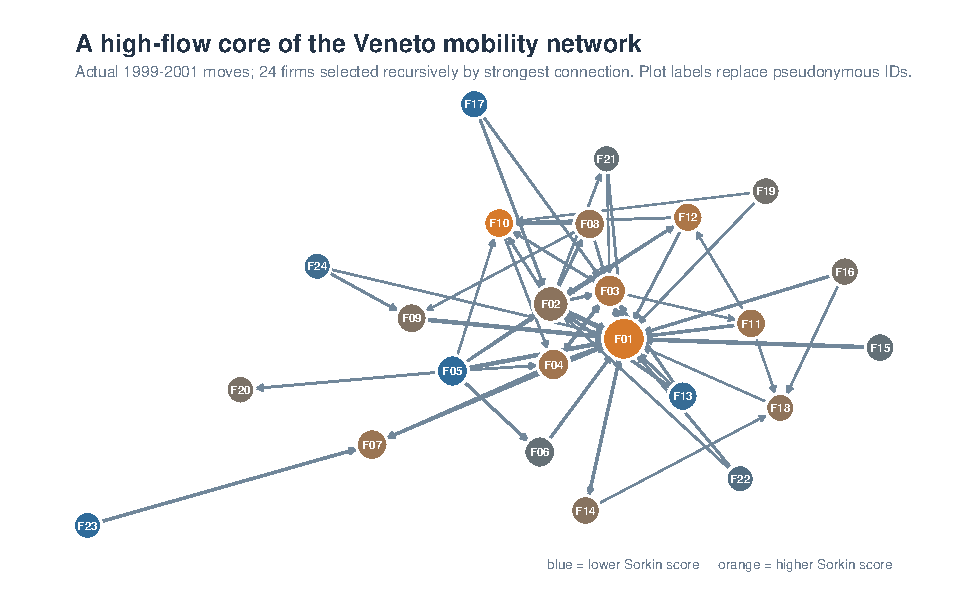
\includegraphics[width=\linewidth]{veneto_network.pdf}
  \caption{An actual high-flow core within the selected Veneto SCC. The plot
  begins with the highest-flow firm and recursively adds the outside firm with
  the strongest connection to the current set until \NetworkNodes{} firms are
  shown; the \NetworkEdges{} highest-flow directed edges among them are drawn.
  Node size reflects total selected-component flow and color reflects the
  Sorkin score. This is a readable subgraph, not the full 702-firm component.}
  \label{fig:veneto-network}
\end{figure}

\subsection{Numerical results}

Both methods satisfy their explicit certificates. Sorkin takes 230 power
iterations; its maximum residual against the original stationary equation is
$1.34\times10^{-11}$. Bradley--Terry takes eight Newton iterations, with a
maximum constrained gradient of $3.51\times10^{-13}$ and no line-search
backtracking.

\begin{table}[htbp]
\centering
\caption{Estimator diagnostics in the Veneto run}
\label{tab:diagnostics}
\small
\begin{tabular}{@{}lrr@{}}
\toprule
Diagnostic & Sorkin & Bradley--Terry \\
\midrule
Iterations & 230 & 8 \\
Fixed-point max residual & 1.34e-11 & -- \\
Fixed-point L1 residual & 9.77e-11 & -- \\
Log likelihood & -- & -1175.084 \\
Maximum score gradient & -- & 3.51e-13 \\
Newton-system residual & -- & 3.51e-13 \\
Line-search backtracks & -- & 0 \\
\bottomrule
\end{tabular}

\end{table}

\begin{figure}[htbp]
  \centering
  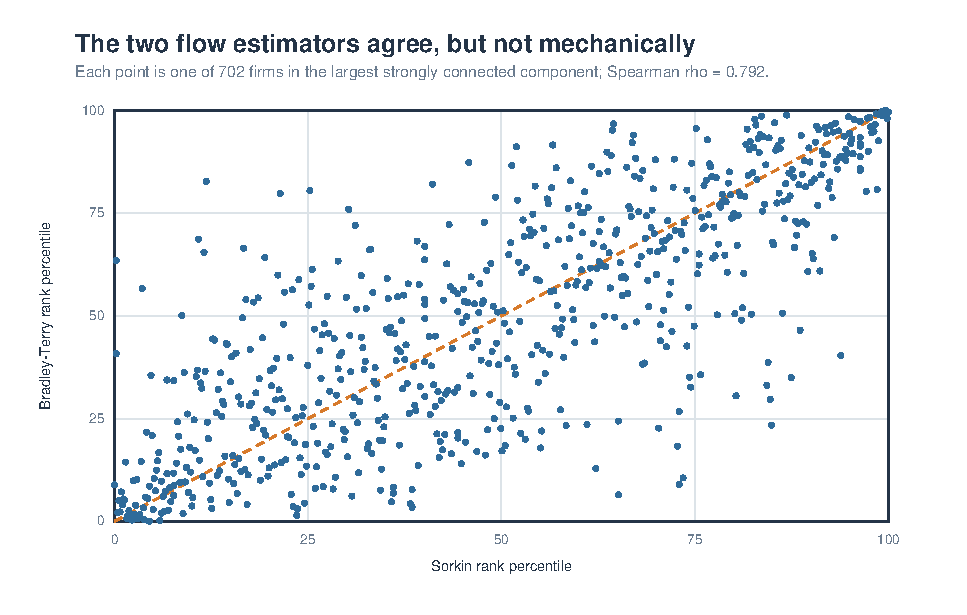
\includegraphics[width=\linewidth]{rank_comparison.pdf}
  \caption{Firm rank percentiles from the two methods. Agreement is strong but
  incomplete because Sorkin propagates flow globally while Bradley--Terry
  conditions on pair comparisons.}
  \label{fig:rank-comparison}
\end{figure}

The methods have a rank correlation of \SorkinBtSpearman{}. Their top deciles
overlap by 60.6 percent. Disagreement is expected: a firm can receive favorable
pairwise outcomes but occupy a different position once flows through the rest
of the network are propagated.

\begin{table}[htbp]
\centering
\caption{Outcomes by decile of the Veneto Sorkin score}
\label{tab:deciles}
\scriptsize
\resizebox{\linewidth}{!}{\begin{tabular}{@{}rrrrrr@{}}
\toprule
Sorkin decile & Firms & Median score & Median BT pct. & Median AKM effect & Total flow \\
\midrule
1 & 70 & -2.997 & 7.8 & 0.0400 & 311 \\
2 & 70 & -1.591 & 26.8 & -0.0131 & 438 \\
3 & 71 & -1.046 & 28.8 & -0.0671 & 367 \\
4 & 70 & -0.544 & 35.2 & 0.0172 & 458 \\
5 & 70 & -0.056 & 42.2 & -0.0078 & 415 \\
6 & 70 & 0.391 & 56.0 & 0.0021 & 494 \\
7 & 70 & 0.835 & 67.2 & 0.0192 & 683 \\
8 & 71 & 1.256 & 69.8 & -0.0211 & 708 \\
9 & 70 & 1.793 & 80.7 & 0.0119 & 401 \\
10 & 70 & 2.760 & 92.8 & 0.0241 & 929 \\
\bottomrule
\end{tabular}
}
\begin{minipage}{\linewidth}\vspace{0.35em}\footnotesize
\emph{Notes:} Decile 10 has the highest Sorkin scores. Bradley--Terry (BT) is
reported as a rank percentile. The AKM-style effect uses the supplied outcome
and is centered across the 702 firms. Total flow is inflow plus outflow summed
over firms and therefore counts each within-component move twice.
\end{minipage}
\end{table}

\subsection{A transparent AKM-style comparison}
\label{subsec:akmcompare}

To make the distinction from familiar wage decompositions concrete, the
replication estimates a narrow two-period first-difference benchmark on
workers whose origin and destination firms both belong to the selected SCC:
\begin{equation}
  \Delta y_w=\delta+\psi_{J_{w,2001}}-\psi_{J_{w,1999}}+u_w.
  \label{eq:akm-diff}
\end{equation}
This eliminates a time-invariant worker effect as in a two-period AKM model.
Same-firm workers help estimate the common period change $\delta$, while movers
identify differences in $\psi$. The benchmark uses \AkmRows{} worker
transitions, of which \AkmMovers{} are movers; a sparse conjugate-gradient solve
converges in \AkmIterations{} iterations. The estimated common change is
\AkmPeriodEffect{} in the supplied outcome's units and the regression
$R^2$ is \AkmRSquared{}.

This is an illustration, not a replacement for a production AKM analysis. It
has two periods, no controls, no leave-out correction, and no attempt to model
limited mobility bias. The public file's fourth column is treated generically
as the supplied outcome. The comparison is useful precisely because
\texttt{ferank} does not read that column.

\begin{figure}[htbp]
  \centering
  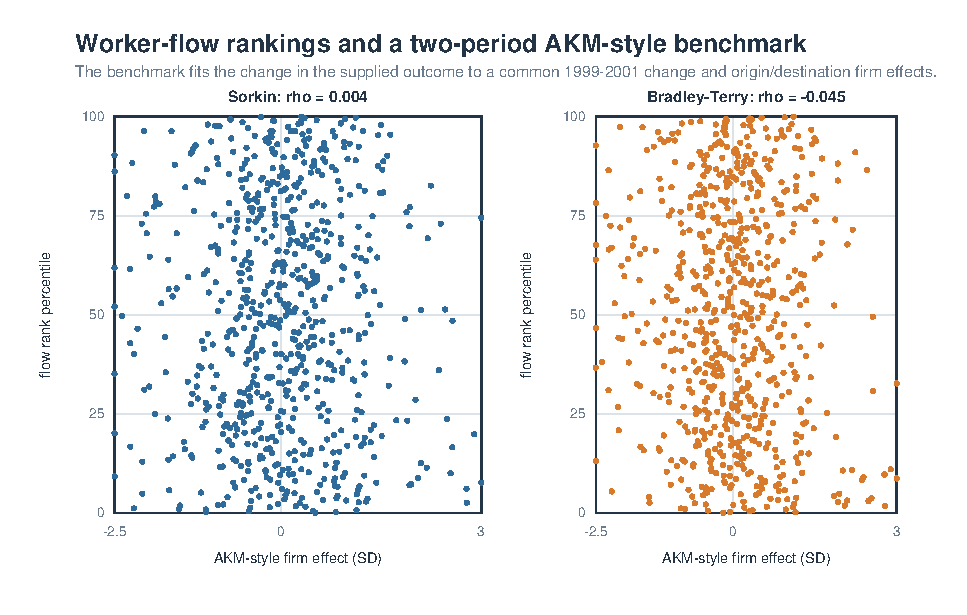
\includegraphics[width=\linewidth]{akm_comparison.pdf}
  \caption{The flow ranks are essentially unrelated to this narrow outcome
  benchmark in the public teaching extract. Boundary points reflect clipping
  at the first and ninety-ninth percentiles of the standardized benchmark for
  legibility. This pattern is not evidence that either estimator is wrong;
  they summarize different moments of the data.}
  \label{fig:akm-comparison}
\end{figure}

\begin{table}[htbp]
\centering
\caption{Agreement among the Veneto scores and outcome benchmark}
\label{tab:agreement}
\small
\begin{tabularx}{\linewidth}{@{}Xrr@{}}
\toprule
Comparison & Pearson & Spearman \\
\midrule
Sorkin vs. Bradley--Terry score & 0.781 & 0.792 \\
Sorkin score vs. AKM-style effect & -0.017 & 0.004 \\
Bradley--Terry score vs. AKM-style effect & -0.092 & -0.045 \\
\addlinespace
Top-decile overlap (share of Sorkin top decile) & \multicolumn{2}{r}{0.606} \\
\bottomrule
\end{tabularx}

\end{table}

In this extract, the Sorkin and AKM-style rank correlation is
\SorkinAkmSpearman{}, and the Bradley--Terry and AKM-style rank correlation is
\BtAkmSpearman{}. The substantive lesson is not that flow rankings should
always be orthogonal to wage effects. It is that their empirical relationship
is an estimable fact, not a definition. Job flows may reflect wages, amenities,
geography, search frictions, worker composition, hiring opportunities, firm
size, and the construction of employment spells.

\section{A practical empirical workflow}
\label{sec:workflow}

For an applied project, the following sequence keeps graph construction and
interpretation auditable:
\begin{enumerate}
  \item \textbf{Define employment spells first.} Resolve concurrent jobs,
  nonemployment, recalls, and the time unit before calling the command.
  \item \textbf{Tabulate the transition accounting.} Record input rows, valid
  transitions, gap breaks, missing-firm breaks, same-firm continuations, moves,
  graph firms, edges, SCCs, and selected firms.
  \item \textbf{Inspect sensitivity to graph rules.} Re-run defensible
  \texttt{maxgap()} and \texttt{minflow()} choices. Changes in the largest SCC
  are part of the estimand, not merely a nuisance.
  \item \textbf{Run both methods when useful.} Agreement is informative;
  disagreement reveals the distinction between global propagation and
  pair-conditional wins.
  \item \textbf{Check certificates, not just ranks.} Save
  \texttt{estat convergence}, graph coverage, and generated variables.
  \item \textbf{Check mapped coverage and weighting.} Missing generated values
  identify selected observations without ranked firms. Use one observation
  per firm for equal-firm summaries; worker-year rows induce person-year weights.
  \item \textbf{Name the estimand precisely.} Keep descriptive worker-flow
  rankings separate from wage effects and causal claims.
\end{enumerate}

\section{Returned results and reproducibility}
\label{sec:returns}

The most frequently used \texttt{e()} results are summarized with their
Veneto values in \cref{tab:returns}. Additional scalars include gap and
missing-firm breaks, numerical timing, method-specific residuals, Newton
diagnostics, and requested thread count.

\begin{table}[htbp]
\centering
\caption{Selected stored results after the Veneto run}
\label{tab:returns}
\small
\begin{tabularx}{\linewidth}{@{}lR{0.18\linewidth}X@{}}
\toprule
Returned result & Veneto value & Meaning \\
\midrule
\texttt{e(N\_input)} & 71,614 & Input rows after markout \\
\texttt{e(N\_firms)} & 3,630 & Firms in the informative mobility graph \\
\texttt{e(N\_results)} & 702 & Firms returned after component selection \\
\texttt{e(N\_edges)} & 6,043 & Canonical directed edges before selection \\
\texttt{e(N\_components)} & 2,917 & Strongly connected components \\
\texttt{e(valid\_moves)} & 8,243 & Cross-firm transitions \\
\texttt{e(same\_firm\_continuations)} & 27,564 & Valid adjacent records without a move \\
\texttt{e(method)} & method name & Estimator actually run \\
\texttt{e(component)} & largest & Component rule actually applied \\
\texttt{e(normalize)} & mean & Score normalization \\
\bottomrule
\end{tabularx}

\end{table}

The complete report build is driven by
\texttt{report/replication/run\_report.sh}. It:
\begin{enumerate}
  \item downloads or copies the public example and verifies its exact hash;
  \item builds the native macOS plugin from the pinned Rust sources;
  \item runs both Stata estimators and requires an explicit PASS marker;
  \item generates only aggregate, disclosure-safe vector figures and tables;
  and
  \item compiles this document with \texttt{latexmk}.
\end{enumerate}
Raw teaching data, Stata result CSVs, logs, LaTeX intermediates, and the compiled
PDF are excluded from version control. The script accepts
\texttt{FERANK\_VENETO\_SOURCE} for an existing local CSV or CRAN archive.

\section{Concluding interpretation}

For an AKM-trained economist, graph theory adds one essential piece of
information: direction. Undirected connectedness tells us where relative firm
effects can be linked through movers. Directed strong connectedness tells us
where a finite, mutually comparable worker-flow ranking exists without an
invented bridge. Sorkin and Bradley--Terry then use the same arrows in different
ways---one through a global stationary system, the other through pairwise
destination wins.

The Veneto teaching example makes all three layers visible. Panel rules create
\VenetoMoves{} moves; graph rules reduce \VenetoGraphFirms{} mobility firms to
a largest SCC of \VenetoLargestSCC{} firms; estimator rules yield two related
but distinct rankings. The numerical certificates say the stated equations
were solved accurately. They do not convert the resulting descriptive scores
into wage effects or causal employer values. That final distinction is the
most important one to preserve in empirical use.

\appendix
\section{Derivations and numerical details}

\subsection{Stationary value as a balance equation}

Combining $\pi=S q$ with $P\pi=\pi$ and $P=MS^{-1}$ gives
\begin{equation}
  Mq=S q.
  \label{eq:sorkin-balance}
\end{equation}
For each firm $i$, revealed value arriving through inward worker flows equals
its outflow exposure times its own revealed value. This form is often the most
direct way to explain the Sorkin fixed point without Markov terminology. The
scale of $q$ is fixed by $\mathbf{1}'Sq=1$; logging turns multiplicative scale
into the additive normalization used for reported scores.

\subsection{Bradley--Terry curvature}

Differentiate \cref{eq:btgradient}. Each compared pair contributes
$w_{ij}(d_i-d_j)^2$ to the quadratic approximation in a proposed score change
$d$. Summing pair contributions produces \cref{eq:laplacian}. Strong
connectivity implies that the undirected comparison graph is connected, so the
only zero-curvature vector is a constant. The mean-zero constraint removes it.

\subsection{Dense reference and sparse production routes}

The bounded \texttt{engine(reference)} implementations separately compute the
stationary vector and constrained Newton solution using dense linear algebra.
They exist for testing, not for large applications. The production engine uses
sparse edge lists throughout. Row permutation, duplicate splitting, firm
relabeling, periodic and nearly reducible chains, extreme logits, separation,
deterministic repetition, and production/reference agreement are covered by
the repository test suite.

\section{Generated-variable contract}

{\small
\begin{longtable}{@{}L{0.31\linewidth}L{0.61\linewidth}@{}}
\toprule
Option & Meaning \\
\midrule
\endfirsthead
\toprule
Option & Meaning \\
\midrule
\endhead
\texttt{generate()} & Descending ordinal midrank; 1 best; exact ties averaged. \\
\texttt{score()} & Normalized log revealed value or Bradley--Terry score; higher better. \\
\texttt{percentile()} & $100(J-\mathrm{rank})/(J-1)$ within each component; equal-firm weights. \\
\texttt{componentid()} & Deterministic canonical SCC ID of the estimated firm. \\
\bottomrule
\end{longtable}
}

Each option takes one new name for a panel, or two names for prepared flows,
origin first. All values are stored as doubles; unselected rows and unmatched
firms have missing values. Component IDs do not make scores across disconnected
groups comparable. Aggregate graph counts, mapping coverage and numerical
certificates are stored in \texttt{e()}; no coefficient vector or public
firm-level result frame is returned.

\begingroup
\small
\setlength{\bibsep}{1.5pt}
\bibliographystyle{plainnat}
\bibliography{references}
\endgroup

\end{document}
